\section{Solving the game exactly}\label{sec:dp}

Part~II searched for a good policy against one opponent. This part computes, for every position, what
happens when \emph{both} sides play perfectly. There is no learning and no sampling: the result is a table,
and Section~\ref{sec:dp-proof} explains why the table is known to be correct. The code is in
\code{perfect\_play/}.

\subsection{The game as a graph}\label{sec:dp-graph}

\begin{definition}[Position]
A position is $x = (T, G, c, n, m)$: the set $T$ of three tiger squares, the set $G$ of goat squares disjoint
from $T$, the number $c \in \{0, \dots, 5\}$ of goats captured, the number $n \in \{0, \dots, 15\}$ of goats placed,
and the side to move $m \in \{\gt, \tg\}$. The goats on the board number $k = |G| = n - c$. The position is in
the \emph{placement phase} if $n < 15$ and in the \emph{movement phase} if $n = 15$.
\end{definition}

The moves are those of Section~\ref{old:2.1}: a goat turn places a goat on an empty square ($n < 15$) or slides
one along an edge ($n = 15$); a tiger turn slides a tiger or captures. $\Succ(x)$ is the set of positions one
legal move after $x$. The game ends in two ways:
\begin{itemize}
\item a capture that brings $c$ to 6 wins for the tigers at once;
\item a side to move with no legal move loses.
\end{itemize}
A game that never ends is a draw. The solved game has no turn limit and no repeat rule;
Section~\ref{sec:dp-limit} adds them back.

Three facts about this graph shape the solution.
\begin{enumerate}
\item \textbf{Captures are permanent.} $c$ never decreases, and in the movement phase neither does $15 - k$.
  A capture leads from $k$ goats on the board to $k - 1$.
\item \textbf{The placement phase cannot repeat.} Every goat turn raises $n$ by one. Ordering positions by
  $(n, m)$ with $(n, \tg) < (n, \gt) < (n + 1, \tg)$, every move goes strictly forward: the placement phase is a
  directed acyclic graph that ends in the movement phase.
\item \textbf{The movement phase can repeat.} Slides are reversible, so with a fixed number of goats the
  positions form a graph with cycles.
\end{enumerate}

\subsection{Counting and indexing the positions}\label{sec:indexing}

Three tigers on 23 squares and $k$ goats on the remaining 20 give $\binom{23}{3}\binom{20}{k} = 1771 \binom{20}{k}$
boards. Positions are grouped in layers:
\begin{align*}
\Lambda^m_k &: \text{movement, } k \in \{10, \dots, 15\} \text{ goats on the board},\ m \text{ to move}, & |\Lambda^m_k| &= 1771 \tbinom{20}{k}, \\
\Pi^m_n &: \text{placement, } n \in \{0, \dots, 14\} \text{ placed},\ m \text{ to move}, & |\Pi^m_n| &= \sum_{c=0}^{\min(n, 5)} 1771 \tbinom{20}{n - c}.
\end{align*}
The totals are
\[
2 \sum_{k=10}^{15} 1771 \tbinom{20}{k} = 2{,}162{,}284{,}740 \ \text{(movement)}, \qquad
2 \sum_{n=0}^{14} |\Pi^{\gt}_n| = 16{,}855{,}634{,}180 \ \text{(placement)},
\]
together $19{,}017{,}918{,}920$ positions. Every arrangement is included, whether or not a game can reach it
(Section~\ref{sec:longest} deals with that).

A table needs each board to have an address. The \textbf{combinatorial number system} gives one. Write the
tiger squares as $t_1 < t_2 < t_3$. Renumber the 20 other squares $0, \dots, 19$ in increasing order and write the
goats' new numbers as $j_1 < \dots < j_k$. Then
\begin{equation}\label{eq:rank}
\operatorname{rank}(T, G) = \Big[\tbinom{t_1}{1} + \tbinom{t_2}{2} + \tbinom{t_3}{3}\Big] \tbinom{20}{k} + \sum_{i=1}^{k} \tbinom{j_i}{i}
\end{equation}
is a bijection from the boards with $k$ goats onto $\{0, \dots, 1771\binom{20}{k} - 1\}$. Its inverse peels off the
largest binomial coefficient at each step. \code{prove\_rules.py} checks the round trip on every one of the
$\sum_{k=0}^{15} 1771 \binom{20}{k} = 1{,}846{,}054{,}980$ indices. Inside a placement layer the blocks for
$c = 0, 1, \dots$ follow each other, each indexed by \eqref{eq:rank} with $k = n - c$.

\subsection{Values and the recursion}\label{sec:dp-values}

\begin{definition}[Win and loss in $j$ plies]\label{def:wl}
For the side to move, define sets $\Lo_0, \W_1, \Lo_2, \W_3, \dots$ in order of $j$:
\begin{itemize}
\item $x \in \Lo_0$ if $x$ has no legal move.
\item $x \in \W_j$ ($j \ge 1$) if $x$ is in no earlier set and has a move that wins at once (the 6th capture,
  $j = 1$) or a move to a position in $\Lo_{j-1}$.
\item $x \in \Lo_j$ ($j \ge 2$) if $x$ is in no earlier set, has a legal move, every move leads to a position in
  some $\W_i$ with $i < j$, and at least one leads to $\W_{j-1}$.
\end{itemize}
The \textbf{value} is $v(x) = \W$ if $x \in \bigcup_j \W_j$, $v(x) = \Lo$ if $x \in \bigcup_j \Lo_j$, and $v(x) = \D$ (draw)
otherwise. For $v(x) \neq \D$ the \textbf{distance} $d(x)$ is the index $j$ of the set containing $x$.
\end{definition}

The definition says what it should. From a position in $\W_j$ the mover can end the game with a win in at
most $j$ plies whatever the opponent does, and no faster against the best defence. From a position in
$\Lo_j$ the mover loses within $j$ plies and can last exactly that long. Wins have odd $j$ and losses even
$j$, because the winner makes the last move. A drawn position is one from which neither side can force a
win in any number of plies.

Equivalently, $v$ and $d$ satisfy the \textbf{minimax recursion} at every position $x$ with a legal move:
\begin{equation}\label{eq:minimax}
\begin{aligned}
v(x) &= \begin{cases}
\W & \text{if some } y \in \Succ(x) \text{ has } v(y) = \Lo, \text{ or a move wins at once} \\
\Lo & \text{if every } y \in \Succ(x) \text{ has } v(y) = \W \\
\D & \text{otherwise}
\end{cases} \\[0.4em]
d(x) &= \begin{cases}
1 + \min\{d(y) : y \in \Succ(x),\ v(y) = \Lo\} & v(x) = \W \quad (\text{1 for a move that wins at once}) \\
1 + \max\{d(y) : y \in \Succ(x)\} & v(x) = \Lo
\end{cases}
\end{aligned}
\end{equation}
The winner takes the shortest way and the loser the longest. This is the Bellman equation of the game. It is
the two-player, undiscounted counterpart of the equation for $V^\pi$ in Section~\ref{sec:fp-mdp}, with
$\max$ and $\min$ in place of the expectation.

\begin{remark}[Why the ply counts matter]\label{rem:cycles}
On a graph with cycles, the first line of \eqref{eq:minimax} alone does not determine $v$. Take two positions
that can only move to each other. Labelling one $\W$ and the other $\Lo$ satisfies the value equations,
although the true value of both is a draw. The distances rule this out: they would need $d(x) = 1 + d(y)$ and
$d(y) = 1 + d(x)$. Carrying exact ply counts is therefore what makes a table checkable
(Theorem~\ref{thm:certificate}), not just a refinement.
\end{remark}

\subsection{Movement phase: retrograde analysis}\label{sec:dp-movement}

The movement layers are solved in the order $k = 10, 11, \dots, 15$ (five captures first). When layer $k$ is
solved, layer $k - 1$ is already known, so every capture leads to a position with a known value. Inside the
layer, cycles rule out a simple backward pass. \textbf{Retrograde analysis} works outward from the positions
whose value is known, in order of distance (Algorithm~\ref{alg:retro}).

\begin{algorithm}[H]
\caption{Retrograde analysis of one movement layer $k$ (both sides to move)}\label{alg:retro}
\begin{tabbing}
\hspace{1.6em}\=\hspace{1.6em}\=\hspace{1.6em}\=\kill
\textbf{Initialize} every position $x$ of the layer: \\
\> no legal move: label $x$ as lost in 0 \\
\> otherwise: $\text{open}(x) \leftarrow$ number of moves that stay in the layer or capture into a drawn position \\
\> tigers to move: from the captures of $x$ into layer $k - 1$ (or the 6th capture) record \\
\>\> $e_{\W}(x)$ = fastest win through a capture ($1$ for the 6th capture; $1 + d(y)$ for $y$ lost; none if absent) \\
\>\> $e_{\Lo}(x)$ = largest $d(y)$ over captures into positions $y$ the goats win \\
\> tigers to move with $\text{open}(x) = 0$ and no winning capture: label $x$ as lost in $1 + e_{\Lo}(x)$ \\
\textbf{for} level $j = 0, 1, 2, \dots$ until no position is labelled with distance $\ge j$: \\
\> \textbf{for} every position $y$ labelled with distance $j$, and every $x$ in the layer with a slide to $y$: \\
\>\> $y$ is lost: if $x$ is unlabelled, label $x$ as won in $j + 1$ \\
\>\> $y$ is won: $\text{open}(x) \leftarrow \text{open}(x) - 1$; if it reaches 0 and $x$ has no winning capture, \\
\>\>\> label $x$ as lost in $1 + \max(j,\ e_{\Lo}(x))$ \\
\> \textbf{for} every unlabelled tiger position $x$ with $e_{\W}(x) = j + 1$: label $x$ as won in $j + 1$ \\
\textbf{Every position still unlabelled is a draw.}
\end{tabbing}
\end{algorithm}

The predecessors $x$ of $y$ are found by \emph{un-moving}: slides are reversible, so the positions with a slide
to $y$ are obtained by sliding one piece of the side that just moved back to an empty neighbour. Captures
are never un-made, because they are accounted for from the other side, through $e_{\W}$ and $e_{\Lo}$.

\begin{theorem}[Retrograde analysis is exact]\label{thm:retro}
Assume layer $k - 1$ carries the true $(v, d)$. When Algorithm~\ref{alg:retro} stops, every position of layer
$k$ labelled won or lost in $j$ has $v(x) \neq \D$ and $d(x) = j$ with that result, and every unlabelled position
has $v(x) = \D$.
\end{theorem}

\begin{proof}
We show by induction on $j$: (a) every label written with distance at most $j$ is correct, and (b) once the
levels below $j$ have been processed, every position with $d(x) \le j$ is labelled.

\emph{Wins.} Let $d(x) = j + 1$, $v(x) = \W$. By \eqref{eq:minimax}, $x$ has a successor $y$ lost in $j$ and none lost
sooner. If $y$ is in the layer, it is labelled before level $j$ is processed by (b), and processing it labels
$x$. If $y$ is reached by a capture, $e_{\W}(x) = j + 1$ and the last line of the loop labels $x$. No earlier level
labels $x$ as won, since that would need a successor lost sooner. And $x$ is never labelled lost: a lost
successor in the layer is never subtracted from $\text{open}(x)$, and a winning capture blocks the loss label.
Conversely a win label $j + 1$ is written
only when a successor lost in $j$ exists, and only if no smaller label was written first, so it is the
minimum.

\emph{Losses.} Let $d(x) = j + 1$, $v(x) = \Lo$. Every successor is won with distance at most $j$, one of them
exactly $j$. Each successor in the layer decrements $\text{open}(x)$ when its level is processed, so the
counter reaches zero when the last, largest in-layer distance $j'$ is processed, and the label is
$1 + \max(j', e_{\Lo}(x)) = j + 1$. Conversely a loss label is written only when every move of $x$ leads to a won
position, with the largest of their distances.

\emph{Draws.} By (b), a position with a finite distance is labelled once its level is passed. The loop ends
when no labelled distance remains to be processed, so an unlabelled position has no finite distance: it is in
no $\W_j$ or $\Lo_j$, hence a draw by Definition~\ref{def:wl}. The loop ends because the layer is finite.
\end{proof}

\paragraph{On the GPU.} One thread handles one position: it decodes the index by the inverse of
\eqref{eq:rank}, generates predecessors, encodes them by \eqref{eq:rank}, and writes with atomic operations. A
win is written by compare-and-swap, which succeeds only on an unlabelled entry. Counters are 8-bit fields
decremented atomically. The value is stored in 16 bits: 0 for a draw, $2d$ for a win in $d$, $2d + 1$ for a
loss in $d$. After each layer a separate kernel recomputes \eqref{eq:minimax} for every position from its
successors and compares; it found no disagreement. Table~\ref{tab:mvlayers} gives the result. All six layers
take 22 seconds on an RTX 5070 Ti.

\begin{table}[H]
\centering\footnotesize
\caption{Movement phase by layer. $c = 15 - k$ goats are captured. ``Win'' and ``loss'' are for the side to
move; ``max'' is the largest distance $d$ in plies.}\label{tab:mvlayers}
\begin{tabular}{@{}rrr rrrr rrrr@{}}
\toprule
 & & & \multicolumn{4}{c}{goats to move} & \multicolumn{4}{c}{tigers to move} \\
\cmidrule(lr){4-7}\cmidrule(l){8-11}
$k$ & $c$ & boards & win & loss & draw & max & win & loss & draw & max \\
\midrule
\tabin{generated/tab_movement_layers}
\bottomrule
\end{tabular}
\end{table}

With no captures ($k = 15$) the goats win 69\% of the positions in which they are to move and never lose.
With five captures ($k = 10$) they lose 60\%. The tigers have no forced win in any movement position with
fewer than two captures.

\subsection{Placement phase: backward induction}\label{sec:dp-placement}

The placement phase is acyclic (Section~\ref{sec:dp-graph}), so one pass in reverse order solves it:
\[
\Lambda^{\tg}_{15 - c} \ \to\ \Pi^{\gt}_{14} \ \to\ \Pi^{\tg}_{14} \ \to\ \Pi^{\gt}_{13} \ \to\ \dots \ \to\ \Pi^{\gt}_{0} \ \to\ \Pi^{\tg}_{0}.
\]
A goat placement from $\Pi^{\gt}_n$ leads to $\Pi^{\tg}_{n+1}$ (or, for $n = 14$, to the movement layer
$\Lambda^{\tg}_{15-c}$). A tiger move from $\Pi^{\tg}_n$ leads to $\Pi^{\gt}_n$, in the same block for a slide and in
block $c + 1$ for a capture. Each layer is computed from the one before it by applying \eqref{eq:minimax} once
to every position. Since every successor is already exact, so is the result; no iteration is needed.

Each entry is one byte: 0 for a draw, otherwise $d + 1$. The parity of $d$ tells who wins. The largest
distance is 215, so the byte suffices. The pass takes 27 seconds for 16.9 billion positions.
Table~\ref{tab:pllayers} gives the result.

\begin{table}[H]
\centering\scriptsize
\caption{Placement phase by layer ($n$ goats placed). Positions per side; win and loss are for the side to
move; ``max'' is the largest distance in plies.}\label{tab:pllayers}
\begin{tabular}{@{}rr rrrr rrrr@{}}
\toprule
 & & \multicolumn{4}{c}{goats to move} & \multicolumn{4}{c}{tigers to move} \\
\cmidrule(lr){3-6}\cmidrule(l){7-10}
$n$ & positions & win & loss & draw & max & win & loss & draw & max \\
\midrule
\tabin{generated/tab_placement_layers}
\bottomrule
\end{tabular}
\end{table}

\paragraph{The value of the game.} The opening position is in $\Pi^{\gt}_0$ when the goats move first and in
$\Pi^{\tg}_0$ when the tigers do. Both entries are draws. \textbf{With perfect play neither side can force a win.}

\subsection{Why the tables are correct}\label{sec:dp-proof}

Theorem~\ref{thm:retro} proves the algorithm, not the program. A wrong line of GPU code, a race, or a
misread rule would still give a table. Correctness of the actual files rests on two independent facts.

\paragraph{Fact 1: the table satisfies the recursion everywhere, and that is enough.}

\begin{theorem}[Certificate]\label{thm:certificate}
Let $(\hat v, \hat d)$ assign to every position a value in $\{\W, \D, \Lo\}$ and, when the value is not $\D$, a
finite distance. Suppose that at every position: a position with no legal move has $(\Lo, 0)$; and otherwise
$(\hat v, \hat d)$ satisfies \eqref{eq:minimax} with $\hat v, \hat d$ in place of $v, d$ on both sides. Then
$\hat v = v$ and $\hat d = d$ everywhere.
\end{theorem}

\begin{proof}
\emph{Labelled wins and losses are true, with the right distance}, by induction on $\hat d(x)$. If
$\hat d(x) = 0$ then $x$ has no move and is truly lost in 0. If $\hat v(x) = \W$ with $\hat d(x) = j$, then by
\eqref{eq:minimax} some successor $y$ has $(\Lo, j - 1)$ and none has $\Lo$ with a smaller distance. By
induction $y$ is truly lost in $j - 1$, so $x$ is won in at most $j$. If $x$ were won faster, it would have a
successor truly lost in fewer than $j - 1$ plies; the second half of the proof shows that such a position is
labelled $\Lo$ with that distance, a contradiction. The case $\hat v(x) = \Lo$ is the same with $\max$.

\emph{True wins and losses are labelled}, by induction on the true distance $d(x)$. If $d(x) = 0$ the label is
$(\Lo, 0)$ by assumption. If $x$ is truly won in $j$, it has a successor truly lost in $j - 1$, which by
induction is labelled $(\Lo, j - 1)$; then \eqref{eq:minimax} forces $\hat v(x) = \W$, and by the first half the
distance is $j$. If $x$ is truly lost in $j$, all its successors are truly won within $j - 1$ plies and by
induction labelled so; then \eqref{eq:minimax} forces $(\Lo, j)$.

\emph{Draws.} A position labelled $\D$ is not truly won or lost, by the second half. A position truly drawn is
not labelled $\W$ or $\Lo$, by the first half.
\end{proof}

The theorem turns correctness into a local property that can be checked position by position, with no need
to trust how the table was made. \code{check\_all.py} does exactly that for all 19{,}017{,}918{,}920 entries. It
was written separately from the solver, from the rules and the file format only, and runs on the CPU. It
found \textbf{no mismatch}. As a test of the checker itself, 50 deliberately corrupted entries were all reported.

\paragraph{Fact 2: the rules used are the environment's rules.} The checker and the solver could share a
misunderstanding of the game. \code{prove\_rules.py} excludes that by comparing both with \code{TnGEnv} itself,
exhaustively rather than by sampling. The argument is one of locality:
\begin{enumerate}
\item The moves of a piece depend only on squares near it. This is not assumed. Every board square that the
  environment's move code reads is recorded, per piece, and every read lies within two steps of the piece
  (or on a hub landing square).
\item All 433{,}127 distinct local patterns are enumerated, and on each the environment's legal moves and
  capture effects equal those of the solver's rules.
\item Hence the two agree on every board, since any board is a combination of local patterns already
  checked.
\item The checker's move generator equals the solver's on all 1{,}846{,}054{,}980 boards, by direct comparison.
\end{enumerate}

\paragraph{The rule correction this found.}\label{sec:rulefix} Step 2 failed on 1{,}248 patterns at first, all
of one kind: a tiger on \code{d1} (square 4) jumping a goat on \code{c1} (3) to \code{b1} (2). The environment's
function that decides which goat a capture removes matched the path $4 \to 0 \to 2$ through the hub first. It
therefore removed the goat on the hub if there was one, and otherwise none, leaving the jumped goat in
place. The move list was right; only the removal was wrong. \code{env\_tng.py} was corrected on this branch,
and the tables describe the corrected rule. Models trained before the correction saw the old behaviour;
Section~\ref{sec:cmp-fix} measures what that cost them.

\begin{table}[H]
\centering\small
\caption{What establishes the tables.}\label{tab:verification}
\begin{tabular}{@{}p{0.50\linewidth}p{0.26\linewidth}p{0.17\linewidth}@{}}
\toprule
Check & Scope & Result \\
\midrule
Recursion \eqref{eq:minimax} with distances, independent CPU checker & all 19{,}017{,}918{,}920 positions & 0 mismatches \\
Legal moves and capture effects, environment vs.\ solver rules & all 433{,}127 local patterns & 0 mismatches \\
Index bijection \eqref{eq:rank} & all 1{,}846{,}054{,}980 indices & 0 failures \\
Checker's rules vs.\ solver's rules & all 1{,}846{,}054{,}980 boards & 0 mismatches \\
Recursion recomputed on the GPU during the solve & all movement positions & 0 failures \\
Values and distances recomputed in plain Python & 126{,}000 random positions & 0 mismatches \\
Perfect player against scripted and trained opponents & 1{,}200 games in \code{TnGEnv}, 5{,}600 in Section~\ref{sec:comparisons} & never lost \\
\bottomrule
\end{tabular}
\end{table}

\subsection{The turn limit and the repeat rule}\label{sec:dp-limit}

\code{TnGEnv} ends a game after $\knob{MAX\_TURNS} = 100$ turns (200 plies), and, when the goats move first,
at the fourth occurrence of a board. Exact ply counts handle both.

\begin{proposition}\label{prop:limit}
Let $x$ be reached after $t$ plies with $v(x) \neq \D$. Under the 200-ply limit the forced result still happens
if and only if $t + d(x) \le 200$. The moves that are optimal without the limit remain optimal with it. The
repeat rule never interrupts a perfect player's win.
\end{proposition}

\begin{proof}
The winner's fastest line needs at most $d(x)$ plies against any defence, and the loser's best defence lasts
$d(x)$ plies. So the game ends by ply $t + d(x)$ and, against best defence, not before; it beats the limit
exactly when $t + d(x) \le 200$. If some move wins in time, the fastest win does; if the loser can outlast the
limit by some move, the slowest loss does. Along a winning line the distance falls by one every ply, so no
position on it can occur twice.
\end{proof}

In the placement phase $t$ is a function of the position: the game has seen $2n$ plies when the goats are to
move and $2n - 1$ when the tigers are, if the goats moved first, and $2n + 1$ and $2n$ if the tigers did. Of
the 4.25 billion placement positions with a forced result, 1{,}316{,}096 (0.03\%) need more plies than the
limit leaves (Figure~\ref{fig:dtm}).

\begin{figure}[H]
\centering
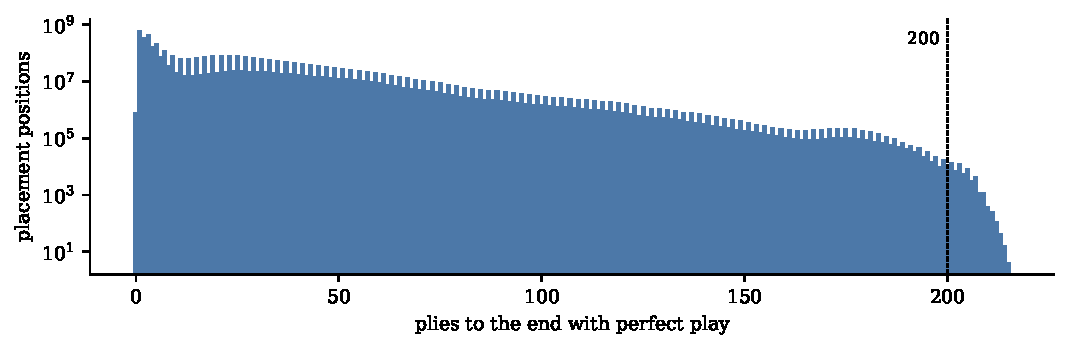
\includegraphics[width=0.95\linewidth]{figures/dtm_histogram.pdf}
\caption{Placement positions with a forced result, by plies to the end (logarithmic scale). Odd distances
are wins for the side to move and even ones losses. Half of these positions end within 9 plies. The count
falls roughly geometrically with the distance, has a shoulder between 160 and 190 plies, and stops at 215.}\label{fig:dtm}
\end{figure}
